\documentclass[crop,tikz]{standalone}
\begin{document}
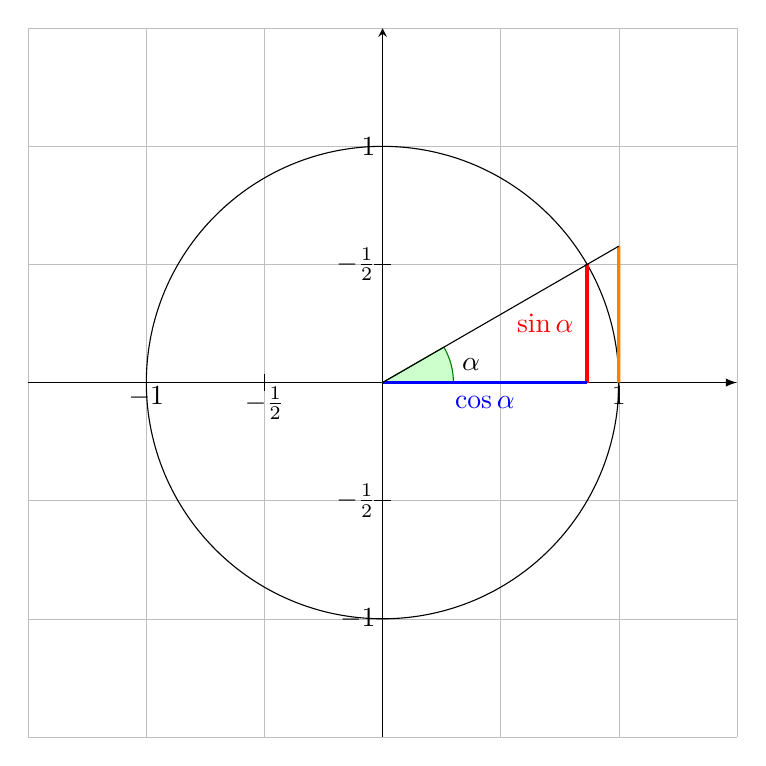
\begin{tikzpicture}[scale=3]
		%\clip[draw] (-0.1,-0.2) rectangle (1.5,1.5);
		\tikzstyle grid_style=[color=gray!50,very thin,step=0.5];
%		\filldraw [gray] (0,0) circle (2pt)
%						 (1,1) circle (2pt)
%						 (2,1) circle (2pt)
%						 (2,0) circle (2pt);
%		\draw (0,0) .. controls (1,1) and (2,1) .. (2,0);
		
		%drawing a circular objects
%		\draw (0,0) circle (10pt);
%		\draw (0,0) ellipse (20pt and 10pt); %20 is the width and 10 is the height
		\draw[style=grid_style] (-1.5,-1.5) grid (1.5,1.5);	
		% drawing in cm and in points
		% AXES 
		\draw[->,>=latex] (-1.5,0)--(1.5,0); %in cm too?
		\draw[->,>=stealth] (0,-1.5)--(0,1.5);

		\foreach \x/\xtext in {-1,-0.5/-\frac{1}{2},1}
			\draw (\x,-1pt) -- (\x,1pt) node[below=1pt]{$\xtext$};

		\foreach \y/\ytext in {-1, -0.5/-\frac{1}{2}, 0.5cm/-\frac{1}{2}, 1}
			\draw (-1pt,\y) -- (1pt,\y) node[left=2pt]{$\ytext$};



		%DRAW CIRCLE
		\draw (0,0) circle (1cm); %START AT (0,0)
%		\draw (0,0) rectangle (0.5,0.5);
%		\draw (-0.5,-0.5) rectangle (-1,-1);
				
		%DRAW ARC
%		\draw (3mm,0mm) arc (0:30:3mm);

		%SHADE AND DRAW
%		\shadedraw[left color=gray, right color=green, draw=green!50!black] (0,0) -- (3mm,0mm) arc (0:30:3mm) -- cycle;
		
		%ADDING ARROW DRAW(LINE) AND FILL
		\filldraw[fill=green!20,draw=green!50!black]
			(0,0) -- (3mm,0mm) arc (0:30:3mm)node[midway,right=0.5pt]{$\alpha$} --cycle;
		
		%DRAW HORIZONTAL AND VERTICAL LINE
		\draw[red,very thick] (30:1cm) -- node[left=1pt]{$\sin \alpha$} +(0,-0.5);
		\draw[blue, very thick] (30:1cm) ++(0,-0.5) -- node[below=1pt]{$\cos \alpha$} (0,0);

		%USING INTERSECTION
		\draw[orange,very thick] (1,0)--(intersection of 1,0--1,1 and 0,0--30:1cm) coordinate (t);
		\draw (0,0) -- (t);
\end{tikzpicture}
\end{document}
